\header{
    \section{Nous sommes unis par la vérole} \label{nous-sommes-unis-par-la-verole}
    %
    
    \insertComment{Première version d'une chanson aussi appelée "Le chant de Lourcine" et datée d'avant 1866}{L'hôpital de Lourcine (de l'Ourcine ou de Saint-Marcel) est un fort ancien hôpital de Paris, déjà abandonné au XVIe siècle, surnommé l'Hôtel-Dieu du Patriarche. Il était situé dans le faubourg Saint Marcel, un faubourg désertique de Paris et abritait les syphilitiques. Après restauration, Henri IV y place les officiers et soldats blessés, où ils sont soignés, logés et nourris. Bien plus tard, sous Louis-Philippe, un second hôpital de Lourcine est créé dans une ancienne abbaye. Ouvert en 1836, il perpétue la tradition de soins aux malades affectés de maladies vénériennes, mais il est cette fois réservé aux femmes.}

    %cf : https://xavier.hubaut.info/paillardes/toubib.htm
}

\enluminure{4}{\href{https://www.youtube.com/watch?v=6xqPPwoC22c}{D}}{e l'hôpital} vieille pratique,
\\Ma maîtresse est une putain
\\Dont le vagin syphilitique
\\Infeste le Quartier Latin.
\\Mais moi, vieux pilier de l'école,
\\Je l'aime à cause de son mal
\\Oui de son mal !
\\Nous sommes unis par la vérole
\\Plus que par le lien conjugal. ~~~~~~~~~~~~~~~~~~~~~\bissimple
\\\\Oui, la vérole nous assemble,
\\Sous les mêmes lois tous les deux
\\Nous vivons, nous souffrons ensemble
\\Plus heureux que des demi-dieux.
\\Tous les matins choquant nos verres
\\Nous y buvons le Van-Swieten
\\Le Van-Swieten !
\\Nous partageons comme des frères
\\Les pilules de Dupuytren. ~~~~~~~~~~~~~~~~~~~~~~~~~~\bissimple
\breakpage
Nous transformons en pharmacie
\\Le lieu sacré de nos amours
\\La valériane et la charpie
\\S'y manipulent tour à tour.
\\Tandis qu'avec de l'iodure,
\\Ma femme me fait des injections
\\Des injections !
\\Avec du chlorure de mercure,
\\Moi, je lui fais des frictions. ~~~~~~~~~~~~~~~~~~~~~~~\bissimple
\\\\Goutte à goutte, de sa matrice
\\Comme d'un alambic fêlé
\\Son urine suinte et glisse
\\Le long de son cul tout pelé.
\\Son con est une casserole
\\Où fermentent en écumant
\\En écumant !
\\La chaude-pisse et la vérole
\\En leur fétide accouplement. ~~~~~~~~~~~~\bissimple
\\\\Sa bouche est un cloaque immonde
\\Toujours buvant, toujours puant
\\Où tous les vits de ce bas monde
\\Ont craché leur foutre gluant.
\\Elle n'est que lèpre et pourriture
\\Et les chiens qui dans le ruisseau
\\Dans le ruisseau !
\\Prendraient sa viande en pâture
\\S'empoisonneraient jusqu'aux os. ~~~~~~\bissimple
\\\\Ses cuisses ont des reflets verdâtres,
\\Ses seins sont flasques et flétris.
\\Dans son con les morpions noirâtres
\\Sur le fumier ont leur logis.
\\Mais moi je l'aime mon amante
\\Et je voudrais jusqu'à demain
\\Jusqu'à demain !
\\Lécher de mes lèvres brûlantes
\\Le foutre de son vieux vagin. ~~~~~~~~~~~~\bissimple
\breakpage
Délassement de l'innocence
\\Je regarde chaque matin
\\Si quelque nouvelle excroissance
\\Ne vient pas orner son vagin.
\\Tandis qu'avec un oeil humide,
\\Elle jette un timide regard
\\Timide regard !
\\Sur mon corps que les syphilides
\\Ont taché comme un léopard. ~~~~~~~~~~~\bissimple
%issu d'autres versions
%Et quand nous serons las de la terre
%\\Nous cesserons tout traitement
%\\Et rongés par un vaste ulcère
\\\\Et quand viendra l'heure dernière,
\\Quand nous s'rons mangés des morpions,
\\Unis dans un dernier ulcère
\\Ad patres nous irons gaiement.
\\Mais nous ferons une supplique
\\Afin qu'nous soyons exposés,
\\Oui exposés !
% issu d'autres versions
%\\Pour être tous les deux portés
%\\Tous deux portés !
\\Dans un musée pathologique
\\À la section des vérolés. ~~~~~~~~~~~~~~~~~~\bissimple
\\
\begin{center}
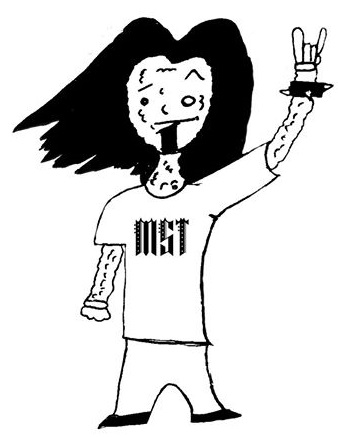
\includegraphics[width=0.6\textwidth]{images/unis_veroles.jpg}
\end{center}

\breakpage